\documentclass{article}
\usepackage[T1]{fontenc}
\usepackage{lmodern}
\usepackage{graphicx}
\usepackage{amsmath,amssymb}
\usepackage[a4paper,margin=2cm]{geometry}
\usepackage[absolute,overlay]{textpos}
\setlength{\TPHorizModule}{1mm}
\setlength{\TPVertModule}{1mm}
\usepackage[indonesian]{babel}
\usepackage{hyperref}
\setlength{\emergencystretch}{2em}
% unit: Halaman 40

\begin{document}

% === Halaman 40 (llm) ===

\vspace{222.16mm}

Cek video \textbf{INTERCEPT ANY RADIO SIGNAL!!!!}: \url{https://www.youtube.com/watch?v=UMu5AhSg-TI}

% deskripsi: Screenshot cuplikan video YouTube yang menunjukkan seseorang memegang perangkat penerima sinyal radio (SDR) dengan tampilan spektrogram.
% bbox normalisasi: [0.0960, 0.1770, 0.6980, 0.9250]
\begin{textblock*}{126.42mm}(20.16mm,52.57mm)
\noindent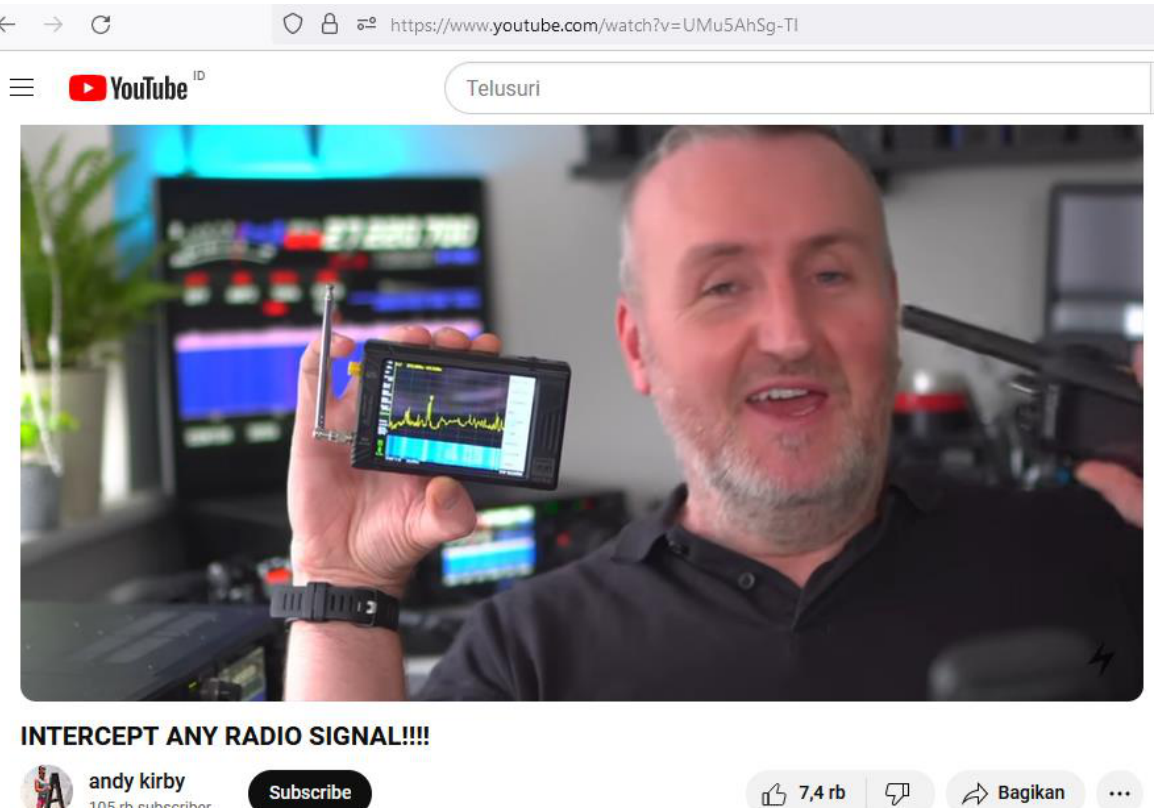
\includegraphics[width=126.42mm,height=222.16mm]{../../images/llm/page_040_img_01.png}%
\end{textblock*}

\end{document}
